\chapter{Marco Teórico}

En este capítulo, son expuestos de manera expédita los conceptos teóricos fundamentales para la comprensión de este trabajo. Se presentan las definiciones de Valor, Emprendimiento, Servicios en Redes Sociales (SNS, por sus siglas en inglés) y Plataforma, así como la descripción esencial de lo que es una aplicación web. Son especificadas las funcionalidades de los entornos de trabajo Vue.js, MongoDB y el servicio de computación en la nube Amazon Web Services (AWS), así como una descripción suscinta de la metodología de la Arquitectura Orientada a Servicios, el Desarrollo Orientado a Funcionalidades y los tableros de tareas Kanban, brindando de esta forma una plataforma teórica que permite al lector apropiarse de una noción de los conceptos acá expuestos y le facilita abordar el contenido expuesto en lo que resta de este proyecto.

\section{Valor}
El Oxford Dictionary ubica el origen etimológico de la palabra valor en valere, que evolucionó hacia el francés antiguo como valoir, que signica “ser de significancia o de importancia”. Para definir al valor de manera suscinta, Kenton (2018) lo describe como la “importancia o valía monetaria, material o de juicio que posee un activo, bien o servicio” \cite{kenton2021}.  Al hablar de valor en el contexto del emprendimiento, Dollinger (2008) plantea el siguiente dilema: “el valor juzga la calidad en términos del precio, y el precio es lo que consideran al momento de adquirir un producto o servicio. Si el dinero no fuese escaso, nada tendría valor, ni siquiera la calidad, porque todos pudiesen comprar cualquier cosa –pero esto, por supuesto, no es cierto. Además, en los negocios donde los precios son señales a las que debemos prestar atención y el dinero es un bien escaso, es el valor, y no la calidad del producto, lo verdaderamente importante” \cite{dollinger2008}. Esto último señala la importancia del valor, concibiéndolo como un índice descriptivo de la valía que le brindan los actores económicos a los productos que yacen en un mercado: por ende, la creación de valor es una de las actividades fundamentales de las sociedades humanas. Una de las actividades esenciales para la creación de valor es el emprendimiento, que como lo describen Mishra y Zachary (2015) consiste en dos fases: la Formulación del Emprendimiento y la Monetización del Emprendimiento. En la primera etapa, el emprendedor inicia con una oportunidad de innovación donde se formula la competencia emprendedora. Muchos emprendimientos fallan en esta etapa. La segunda, por su parte, describe la necesidad de fortalecer un modelo de negocios luego de desarrolladas las competencias de emprendimiento, esto con el objetivo de construir las capacidades dinámicas complementarias requeridas en el proceso emprendedor. Si el emprendimiento es incapaz de obtener mayores inversiones y el modelo de negocios falla, entonces se regresa a la primera etapa.\cite{Mishra2015}


\section{Emprendimiento}

\subsection{Definición}
El término proviene del ya utilizado en el francés a principios del siglo XIX entrepreneur que significa acomerter o comprometerse a realizar algo. La Real Academia Española es bastante explícita cuando define al emprendimiento como: “Acometer y comenzar una obra, un negocio, un empeño, especialmente si encierran dificultad o peligro.” Múltiples autores brindan una serie de definiciones al problema:
Dollinger (2008) realiza un análisis de las distintas definiciones de emprendimiento que radican en la literatura encontrando los siguientes elementos en común:

	Creatividad e Innovación
	Identificación, Adquisición y Clasificación de Recursos
	Organización Económica
	Oportunidad para tener alguna ganancia o incrementarla bajo riesgo e incertidumbre

Considerando estos cuatro elementos, lo define como: “el control y despliegue de recursos para crear una organización económica innovadora con el propósito de generar ganancias o crecimiento bajo condiciones de riesgo e incertidumbre” \cite{dollinger2008}.

\subsection{Objetivos del Emprendimiento}

Las razones que empujan a individuos y organizaciones a tomar la decisión de emprender son muy variadas y particulares. Según lo enunciado en el curso Introduction to Entrepreneurship de Lumen Learning, las motivaciones esenciales pasan por “la independencia financiera, el éxito económico o la búsqueda de un cambio social a una situación negativa”\cite{boundless}.

\subsection{Principios del Emprendimiento}

El emprendimiento al no ser una ciencia o una disciplina regida por una organización o estándar, tiene múltiples principios y fundamentos que lo componen como concepto. Francis Nwokike, emprendedor social, narra en su artículo "10 Principios del Emprendimiento" a partir de sus experiencias en este mundo cuáles deben ser los diez fundamentos y principios que todo emprendedor debe seguir. Los cuales son \cite{principles}:

\begin{enumerate}
	\itemsep1pt \parskip1pt \parsep1pt
	\item Ser un proveedor de soluciones
	\item Tener una visión
	\item Escoger el equipo correcto
	\item Construir un Producto o Servicio Viable
	\item Reducir al mínimo la preocupación por el capital. El capital no escasea, la visión sí.
	\item Ser responsable del éxito o fracaso del negocio
	\item Entender que el crecimiento no es un evento único, es un proceso continuo.
	\item Conocer bien a los clientes
	\item Definir asertivamente las prioridades
	\item Nunca darse por vencido
\end{enumerate}


El término robot alcanza su primera repercusión en la tercera década del siglo pasado, a instancias de R.U.R (\textit{Robots Universal Rossum}), una obra teatral de ciencia ficción escrita por el autor checo Karel Čapek, en la cual por primera vez se hace alusión al concepto de robot, extraído del término checo ``robota'', que significaba ``trabajos forzados''.

A su vez, el término ``robótica'' es acuñado por Isaac Asimov, definiendo a la ciencia que estudia a los robots. Asimov creó también las Tres Leyes de la Robótica, definidas de esta manera:

\begin{enumerate}
	\itemsep1pt \parskip1pt \parsep1pt
	\item Un robot no puede actuar contra un ser humano o, mediante la inacción, permitir que un ser humano sufra daños.
	\item Un robot debe obedecer las órdenes dadas por los seres humanos, salvo que estén en conflictos con la primera ley.
	\item Un robot debe proteger su propia existencia, a no ser que esté en conflicto con las dos primeras leyes.
\end{enumerate}

\section{Plataforma}
El término plataforma viene del francés 
\textit{plateforme} que significa plan de suelo.
Kristjansson et al. (2004) hacen constar que el término plataforma presenta múltiples acepciones y conceptualizaciones a partir del contexto donde se solicite su definición. Así que, tras un estudio donde presentan catorce definiciones distintas, sugieren definir el término plataforma en el contexto del desarrollo de productos como “una colección de componentes principales que son reutilizados para obtener una ventaja competitiva”
\cite{kristjansson2004term}. Múltiples definiciones de la terminación Plataforma se encuentra en la Figura \ref{figure:platformDefinitions}

\begin{figure}[H]
\centering
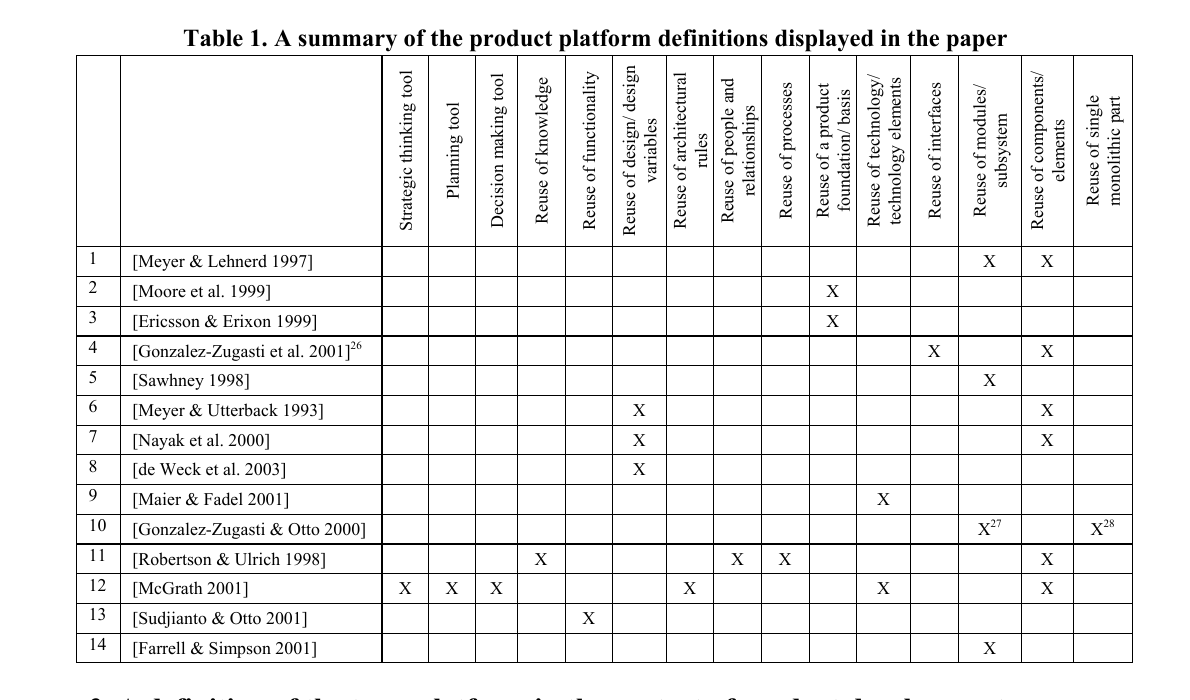
\includegraphics[width=0.80\textwidth]{img/1.png}
\caption{Definiciones de la acepción “Plataforma de producto” mostradas en la literatura \cite{kristjansson2004term}}
\label{figure:platformDefinitions}
\end{figure}

\subsection{Plataformas Digitales}

La Information Technology and Innovation Foundation (ITIF, 2018) define las plataformas digitales como “negocios en línea que facilitan las interacciones comerciales entre al menos dos grupos distintos: los proveedores  y los consumidores”. Facebook, Amazon, Uber o Google entran dentro de la definición de plataformas digitales, pero poseen modelos de negocios distintos, esto genera pues, que las interacciones entre la plataforma misma y los usuarios se den de distintas maneras.
Las plataformas digitales no son algo novedoso, pero ha sido en los últimos años donde se ha extendido su uso gracias a la adopción masiva del internet y al crecimiento de la computación. Hoy en día, poseen una extensa influencia en la economía mundial, aportando alrededor de 2.6 trillones de dólares a la capitalización del mercado.
Las plataformas digitales han reducido de manera drástica los costos y facilitado una amplia gama de transacciones. Un ejemplo de ello ha sido dentro del comercio electrónico (e-commerce), pues alrededor de 360 millones de personas han  participado en alguna transacción. Otro caso documentado ocurrido en la India muestra como el uso de la plataforma proveída por la aplicación WhatsApp ha facilitado a miles de productores rurales la difusión de sus productos a potenciales usuarios.

\subsection{Diseño de Plataformas Digitales}

De Reuver (2018) expone que el entendimiento de las causas del éxito o del fracaso de una u otra plataforma son desconocidas hasta el día de hoy. Sin embargo, los estudios realizados sobre, esencialmente, los casos exitosos, han permitido extraer una serie de condiciones que pueden ayudar a acelerar y a guiar el proceso de diseño de plataformas digitales \cite{deReuver2018}.
Sobre estas condiciones, Bendor-Samuel (2020) explica en su artículo para la revista Forbes “Key To Designing An Effective Digital Platform” que el “78\% de los estudios realizados muestran que las compañías fallan en alcanzar sus objetivos de negocio”. Esto es debido a que las compañías acostumbran a diseñar sus plataformas a grupos homogéneos y categorías en lugar de a los usuarios de manera individual.
Esto permite inferir que la condición esencial para el éxito del diseño elegido de una plataforma digital es que el mismo pueda anteponerse a las necesidades individuales de sus usuarios, y, con base en ello, aumentar su valor \cite{bendorSamuel2020}.

\subsection{Estrategia de Plataformas}

El uso de plataformas como estrategia de creación de valor es descrito en la Guía de Usuario Platform Design Toolkit. En este texto, se delimita un marco conceptual que permite contextualizar e identificar los elementos (llamados entidades) que hacen vida dentro de lo que se conoce como un ecosistema económico, así como plantear dos principios que resultan fundamentales para, según esta estrategia, la creación de valor. En ese sentido, dos conceptos son planteados  como ejes transversales de esta estrategia: el motor de transacciones y el motor de conocimientos.
El motor de transacciones representa el conjunto de canales y contextos que sirven como facilitadores del intercambio de valores entre entidades.
El motor de conocimientos, por su parte, es el conjunto de servicios de soportes y contextos que están desplegados a través de la plataforma para que los participantes sean capaces de aprender, mejorar y evolucionar en sus interacciones \cite{boundarylessplatform} como es visible en la Figura \ref{figure:platformShaper}.

\begin{figure}[H]
\centering
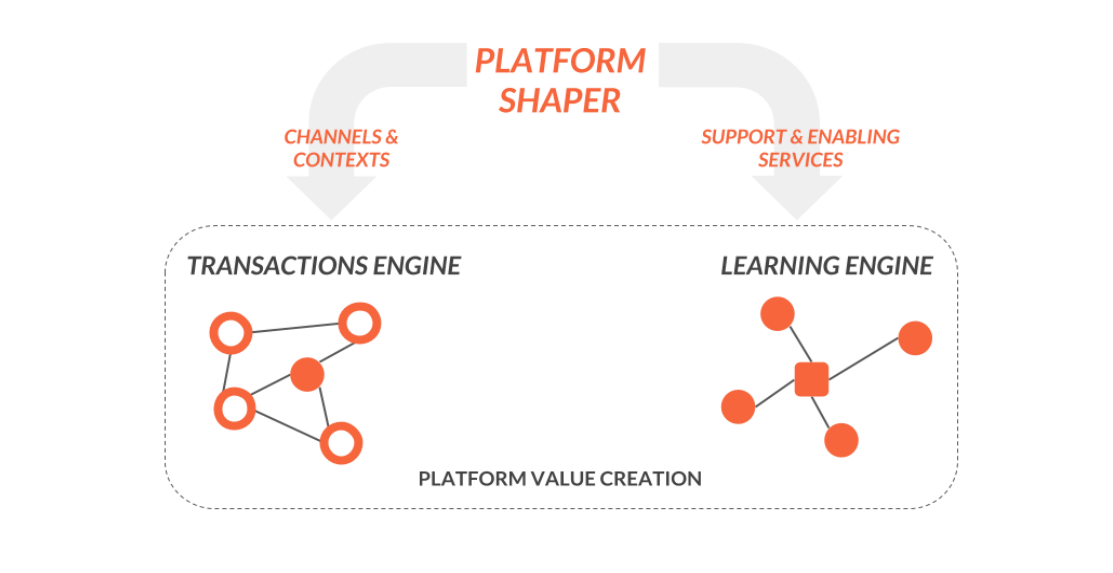
\includegraphics[width=0.80\textwidth]{img/2.png}
\caption{Motores para la Creación de Valor dentro de una plataforma}\cite{boundarylessplatform}
\label{figure:platformShaper}
\end{figure}

\subsubsection{Diseño de una estrategia de plataformas}

Un punto para dar inicio al diseño de plataformas, según la Guía de Usuario Platform Design Toolkit,  es el delimitar el ámbito de la potencial plataforma en un ecosistema. En esencia, este ámbito posee dos espacios internos: un dominio de control, donde la plataforma puede gestionar de manera directa las operaciones de intercambio de valor según sus configuraciones internas, y un dominio de influencia, donde las acciones de la plataforma pueden afectar de manera indirecta otros intercambios de valor. Esto se puede apreciar en la Figura \ref{figure:platformDomain}.

\begin{figure}[H]
\centering
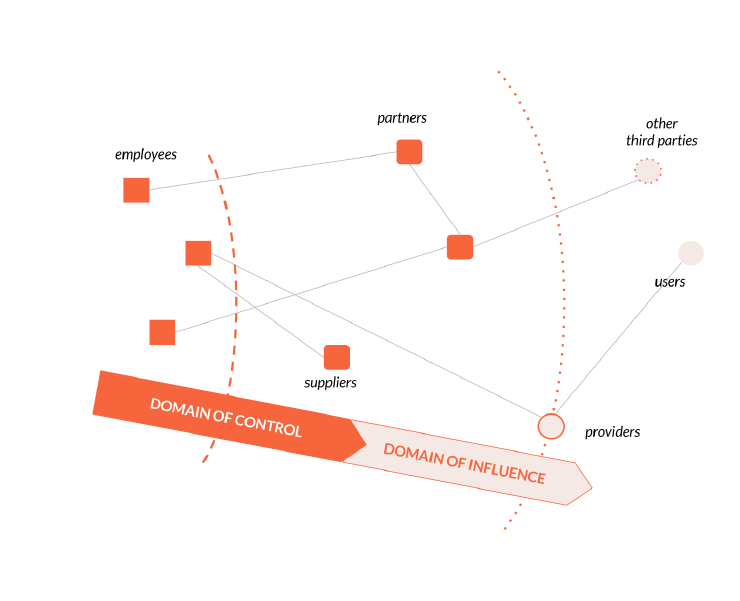
\includegraphics[width=0.80\textwidth]{img/3.png}
\caption{Dominios de Control e Influencia de una plataforma en sus ecosistemas aledaños \cite{boundarylessplatform}}
\label{figure:platformDomain}
\end{figure}

Con esto en mente, existen dos contextos de aplicaciones en los que puede existir una plataforma: la movilización del ecosistema y la innovación del producto y del servicio. En esta dicotomía conceptual, el primer caso busca agregar nuevos ecosistemas a la plataforma a través del desplazamiento de la misma hacia otros ya existentes y bien definidos. El segundo, por su parte, busca captar nuevos ecosistemas a través de la “plataformización” de uno ya existente alrededor de un producto o servicio, como se observa en la Figura \ref{figure:platformSchema}.


\begin{figure}[H]
\centering
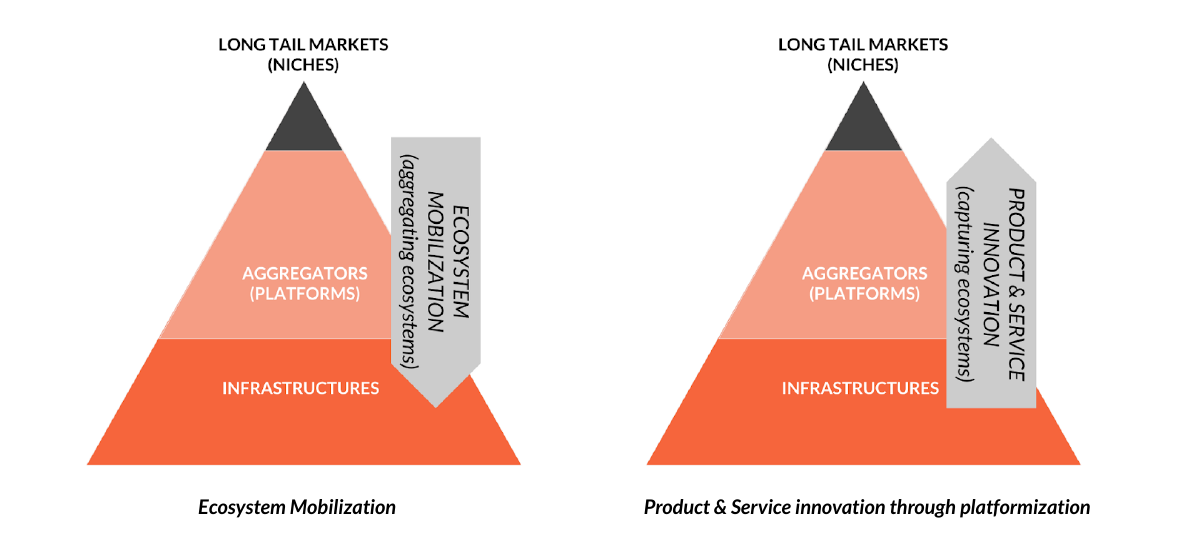
\includegraphics[width=0.80\textwidth]{img/4.png}
\caption{Esquematización de la captura y agregación de ecosistemas \cite{boundarylessplatform}}
\label{figure:platformSchema}
\end{figure}

\section{Servicios en Redes Sociales}

Boloateva y Cata (2010) definen a las redes sociales como plataformas digitales que “permiten a sus usarios comunicarse entre sí, compartir conocimiento acerca de intereses similares, discutir sus temas favoritos, revisar y calificar productos y servicios, entre otros.”
Los Servicios de Redes Sociales son aquellos que, por su propia naturaleza, permiten crear comunidades virtuales y acercamientos entre individuos. Este aspecto general representa potenciales oportunidades en términos de negocios. En este punto, se logran identificar tres grandes oportunidades para el mercadeo: la atención del público con el producto o servicio que se está ofreciendo, el involucramiento de los usuarios de las Redes Sociales en el mercadeo a través de la difusión del contenido, y finalmente el uso de las Redes Móviles para seguir al usuario cuando se encuentre lejos del computador.\cite{bolotaevaCata2011}

\subsection{Características de los Servicios en Redes Sociales}

Si bien las redes sociales pueden aparecer en multitud de formas, todas comparten una serie de características, como el hecho de que todas utilizan internet. Según Kenton (2021), características similares incluyen \cite{kenton2021}:

\begin{itemize}
	\itemsep1pt \parskip1pt \parsep1pt
	\item Contenido generado por el usuario, como fotos, vídeos y publicaciones que informan a otros usuarios sobre actividades e intereses del publicador.
La habilidad de conectar individuos de todo el mundo.
	\item Conectan a las personas con historias comunes, como pueden ser la escuela, el trabajo o simplemente intereses en común.
	\item Pueden ayudar a forjar y desarrollar relaciones entre personas que comparten una profesión o una red de negocios.
	\item Pueden ser utilizadas para ayudar a los individuos a encontrar información, productos, servicios o recursos relevantes para ellos.
\end{itemize}

